\documentclass{homework}
\usepackage{cancel}
\usepackage{amsthm}
\usepackage{cleveref}
\usepackage{upgreek}
\usepackage[framed]{mcode}
\usepackage{mathrsfs}
\usepackage{tikz}
\usepackage{units}
\usetikzlibrary{matrix}
\newtheorem{lemma}{Lemma}

\title{Kevin Joyce}
\course{Math 514 - Inverse Problems - Homework 2}
\author{Kevin Joyce}
\docdate{\today}
\begin{document} 
\newcommand{\figref}[1]{\figurename~\ref{#1}}
\renewcommand{\bar}{\overline}
\renewcommand{\hat}{\widehat}
\renewcommand{\SS}{\mathcal S}
\newcommand{\HH}{\mathscr H}
\newcommand{\mom}{\widetilde}
\newcommand{\mle}{\widehat \Uptheta}
\newcommand{\eps}{\varepsilon}
\newcommand{\todist}{\stackrel{D}\longrightarrow}
\newcommand{\toprob}{\stackrel{p}\longrightarrow}
\newcommand{\TTheta}{\overline{\underline \Theta} }
\newcommand{\del}{\partial}
\newcommand{\approxsim}{\overset{\cdotp}{\underset{\cdotp}{\sim}}}

\begin{longproblem}
  \emph{The Singular Value Decomposition.}  Let $\vect A$ be $m \times n$, with
  $m > n$, and suppose it has singular value decomposition $\vect A = \vect
  {U\Sigma V}^T$. Let $\vect u_i$ be the $i$th column of $\vect U, \vect v_i$
  be the $i$th column of $\vect V$, and $\sigma_i$ the $i$th diagonal element
  of $\vect \Sigma$. 

  \subproblem{ If the rank of $\vect A$ is $r$, show that 
  $$
    \vect A \vect v_i = \begin{cases}
      \sigma_i \vect u_i, & i=1,\dots,r\\
      \vect 0, & i = r+1,\dots,n,
    \end{cases},\quad
    \vect A^T \vect u_i = \begin{cases}
    \sigma_i \vect v_i, & i = 1,\dots,r\\
    \vect 0, & i=r+1,\dots,m.
    \end{cases}
  $$}
  \begin{solution}
    Note that $\vect A \vect v_i = \vect U \vect (\vect \Sigma \vect e_i)  =
    \sigma_i \vect u_i$ and if $r=n$ then the identity above is satisfied.
    Now, suppose $r<n$, then 
    %the set of vectors $\{\vect A\vect v_1,\dots,\vect A \vect v_{r}\} = \{\sigma_1 \vect u_1,\dots,\sigma_{r} \vect u_{r}\}$ is linearly independent, and 
    the set $\{\vect A\vect v_1,\dots,\vect A \vect v_{r+1}\} = \{\sigma_1
    \vect u_1,\dots,\sigma_{r+1} \vect u_{r+1}\}$ is linearly dependent. I.e.
    there exists a non-trivial linear combination so that $x_1\sigma_1\vect u_1
    +\dots+ x_{r+1}\sigma_{r+1}\vect u_{r+1} = \vect0$.  But, by the mutual
    independence of $\vect u_i$, it must be that each scalar product $x_i
    \sigma_i = 0$. Since the singular values are positive and decreasing in
    index, if $\sigma_k = 0$ for $k<r$, then the dimension of the null space of
    $A$ would be greater than $n-r$, violating the rank-nullity theorem.  So each
    $\sigma_1,\dots,\sigma_r$ are strictly greater than zero.  So $x_1,\dots,x_r$ are
    each $0$, and since $(x_1,\dots,x_{r+1})$ is non-trivial, $\sigma_{r+1} = 0$.  Since
    the singular values are positive and decreasing, $\sigma_{r+1} = \dots = \sigma_n = 0$, and
    by the initial observation, $\vect A \vect v_{i} = 0$ for $r<i\le n$. 

    A similar argument follows for the second identity on $\vect A^T$.
  \end{solution}

  \subproblem{Show that
  \begin{equation}
  \vect A = \vect{U\Sigma V}^T \tag{1.20}\label{svd}
  \end{equation}
  can be written $\vect A = \sum_{i=1}^n\vect u_i \sigma_i \vect v_i^T$ and write down the equivalent expression for $\vect A^\dagger$ defined in 
  \begin{equation}
  \vect A^{\dagger} = \vect{V\Sigma}^\dagger \vect U^T.\tag{1.21}\label{pseudo}
  \end{equation}
  }
  \begin{solution}
    We can write
    $$
      \vect\Sigma = \sigma_1 \vect P_1 + \dots + \sigma_n \vect P_n
    $$
    where $\vect P_i$ is the $n\times m$ matrix with 1 in the $(i,i)$th entry and 0 otherwise.  Hence $\vect A = \sum_{i=1}^n\sigma_i\vect U\vect P_i \vect V^T$. Note that the $(i,j)$th entry of 
    $\vect U\vect P_i\vect V^T$ is the scalar product $u_{i,i} v_{j,j}$.  These are precisely the entries of $\vect u_i \vect v_i^T$. We have shown $\vect A = \sum \vect u_i \sigma_i \vect v_i$.  If we recall that the diagonal entries (up to the rank of $A$) of $\vect \Sigma^\dagger$ are $1/\sigma_i$ and zero otherwise, then a similar argument shows that
    $$
      \vect A^\dagger = \vect V \vect \Sigma^\dagger \vect U^T = \sum_{i=1}^{r} \frac 1{\sigma_i}\vect v \vect u^T
    $$
  \end{solution}

  \subproblem{Substitute \eqref{svd} into 
  \begin{equation}
    \vect x_{\mathrm{LS}} = (\vect A^T \vect A)^{-1} \vect A^T \vect b \tag{1.18}\label{leastsq}
  \end{equation}
  To prove
  \begin{equation}
    \vect x_{\mathrm{LS}} = \sum_{i=1} \frac{\vect u_i^T \vect b}{\sigma_i}\vect v_i,\tag{1.22} \label{pseudolstsq}
  \end{equation}
  and hence that $\vect x_{\mathrm{LS}} = \vect A^\dagger\vect b$.
  }
\end{longproblem}
\begin{solution}
  Assuming the columns of $\vect A$ are linearly independent, we carry out the substitution:
  \begin{align*}
  \vect x_{\mathrm{LS}} &= (\vect {V\Sigma}^T \vect U^T \,\vect{U\Sigma V}^T)^{-1} \vect {V\Sigma}^T \vect U^T\vect b\\
  &= \vect {VD}^{-1} \cancel{\vect{ V}^T \,\, \vect V}\vect \Sigma^T \vect U^T\vect b &\text{\small where $D$ is the $n\times n$ diagonal matrix with $\sigma_i^2$ on the diagonal,}\\
  &= \vect V \vect \Sigma^\dagger \vect U^T\vect b &\text{\small since $D \Sigma^T$ has $\sigma_i^{-1}$ as diagonal entries and $0$ otherwise,} \\
  &= \sum_{i=1} \frac{\vect u_i^T \vect b}{\sigma_i}\vect v_i.
  \end{align*}
\end{solution}

\begin{longproblem}
\emph{The discrete Picard condition.} For parts (a)-(d), use \texttt{Deblur1d.m}.  

\subproblem{Create plots verifying that singular vectors of the design matrix $\vect A$ become more oscillatory as $i$ increases. }

\begin{solution}
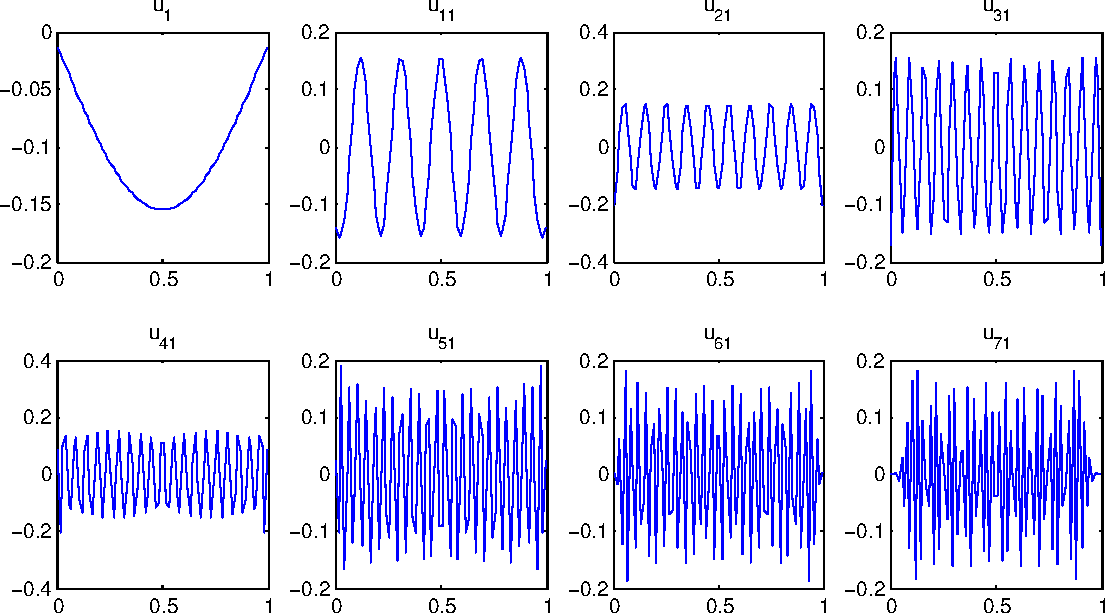
\includegraphics[width=.8\textwidth]{oscillation.pdf}
\end{solution}

\subproblem{A Picard plot for discretized inverse problem is a plot of the values of $\sigma_i$, $|\vect u_i^T\vect b|$, and $|\vect u_i^T \vect b|/\sigma_i$.  For the 1D deblurring example, create the Picard plot, first using the noise-free data and then using noisy data.  Verify in both cases the \emph{discrete Picard condition:} Ignoring the part of the Picard plot where $|\vect u_i^T\vect b|$ levels off due to either numerical round-off (in the noise-free case) or to the presence of noise in $\vect b$, the discrete Picard condition is satisfied if the remaining values of $|\vect u_i^T\vect b|$, on average, decay faster than $\sigma_i$.}

\begin{solution}
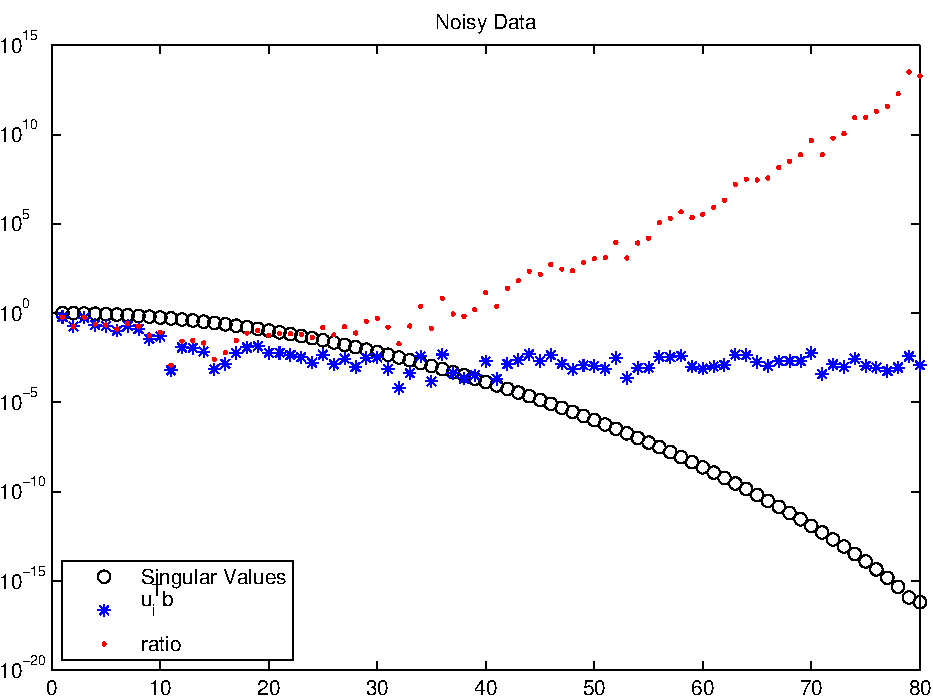
\includegraphics[width=.4\textwidth]{noisy_picard.pdf}
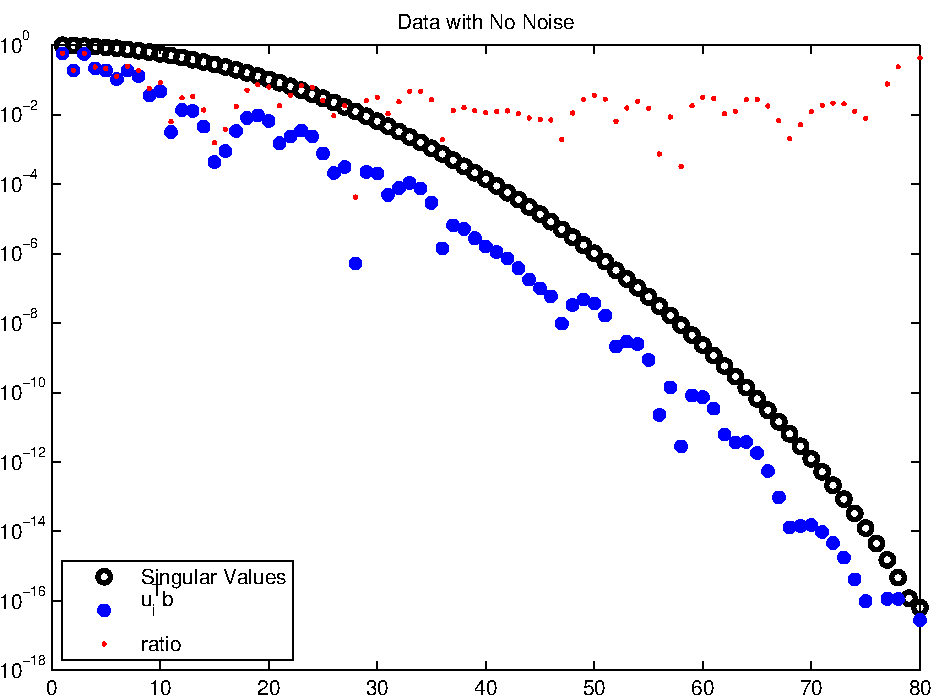
\includegraphics[width=.4\textwidth]{no_noise_picard.pdf}
\end{solution}

\subproblem{Plot the variance values in
\begin{equation}
\vect v_i^T \vect x_{\mathrm{LS}} \sim \mathcal N (\vect v_i^T\vect x, \sigma^3/\sigma_i^2) \tag{1.25}\label{variance}.
\end{equation}
What do they tell you about the statistical properties of the least squares solution.
}
\begin{solution}
\begin{center}
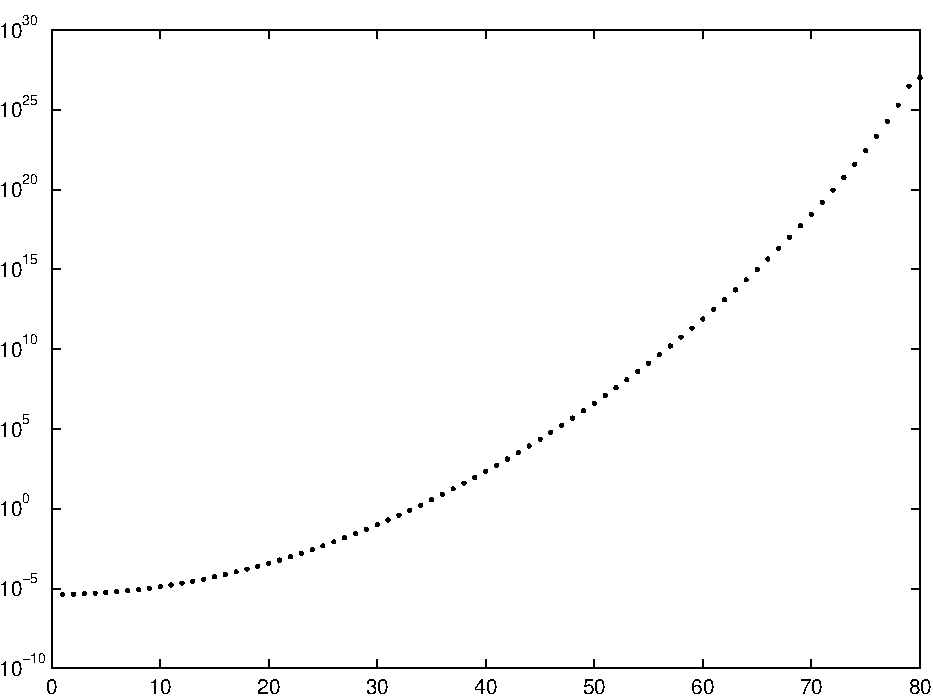
\includegraphics[width=.4\textwidth]{variances.pdf}
\end{center}
The graph above gives the variances of the least squares solution to 1-D deblurring problem projected onto the $i$th left singular vector in the SVD of the debluring discritization -- i.e. the random vector $\vect v^T\vect x_{\mathrm{LS}}$.  The least squares solution, despite being derived from identically distributed data, has coordinates in the basis $\vect v_i$ whose variance grows exponentially as the index $i$ increases as indicated by the graph above.  This means that certain features in the solution (those captured by higher indexed singular vectors) are subject to \emph{extremely high} levels of uncertainty.  In fact, even if the initial noise levels are relatively quite low, any discritization refined finer than 80 or so points will still be corrupted by noise magnification by the apparent exponential growth with the singular vector index which is equal to the number of discritizaiton levels.
\end{solution}

\newpage
\subproblem{Repeat (a)-(c) using \texttt{PSFrecon.m} }

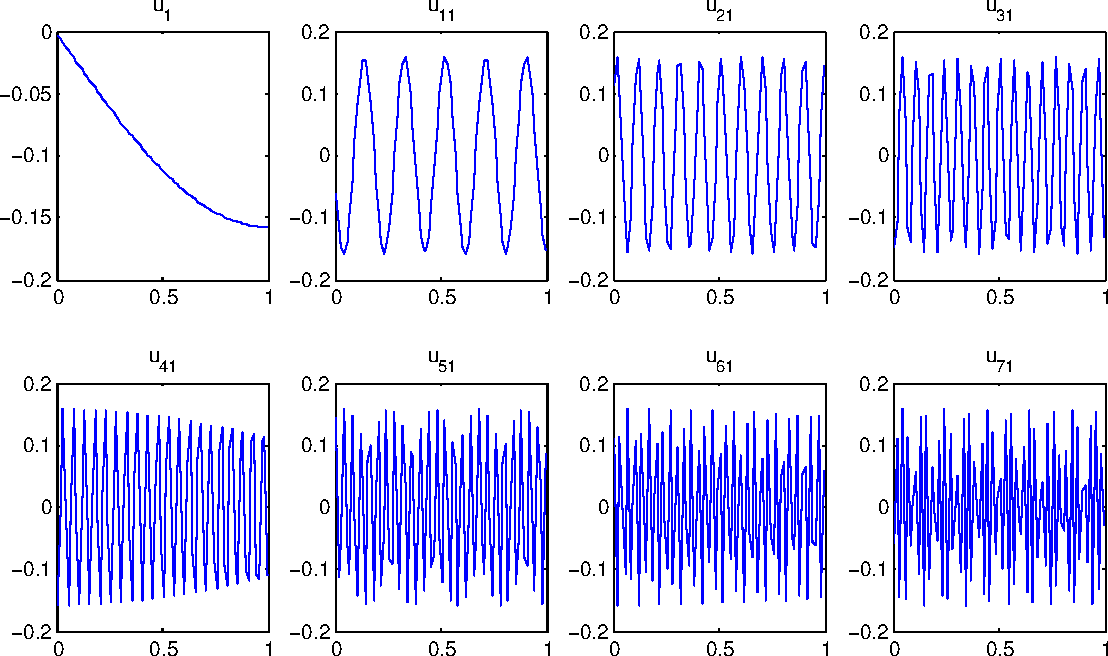
\includegraphics[width=.8\textwidth]{oscillation2.pdf}

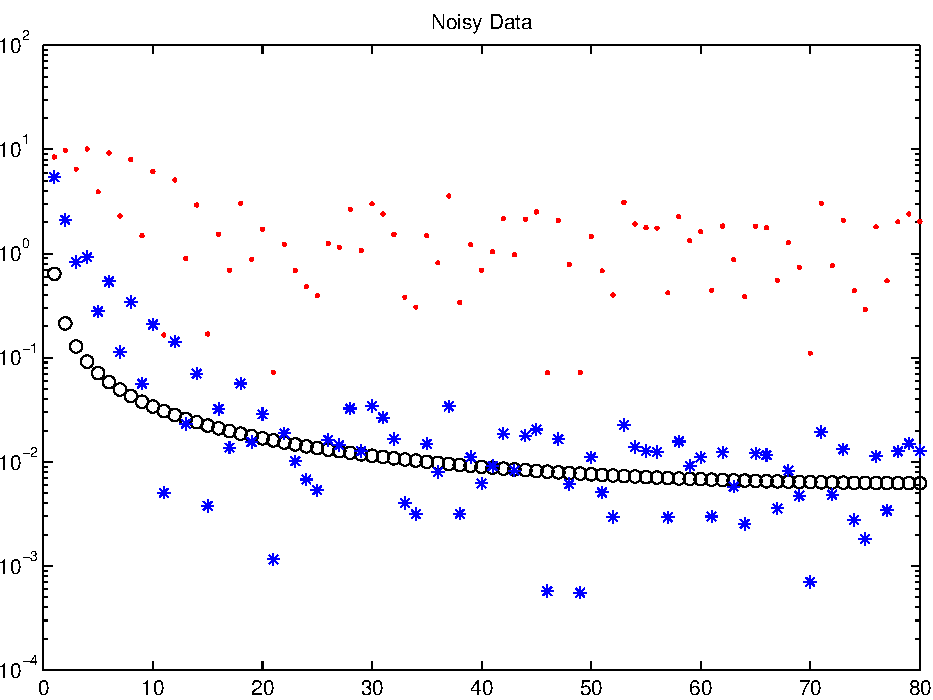
\includegraphics[width=.4\textwidth]{noisy_picard2.pdf}
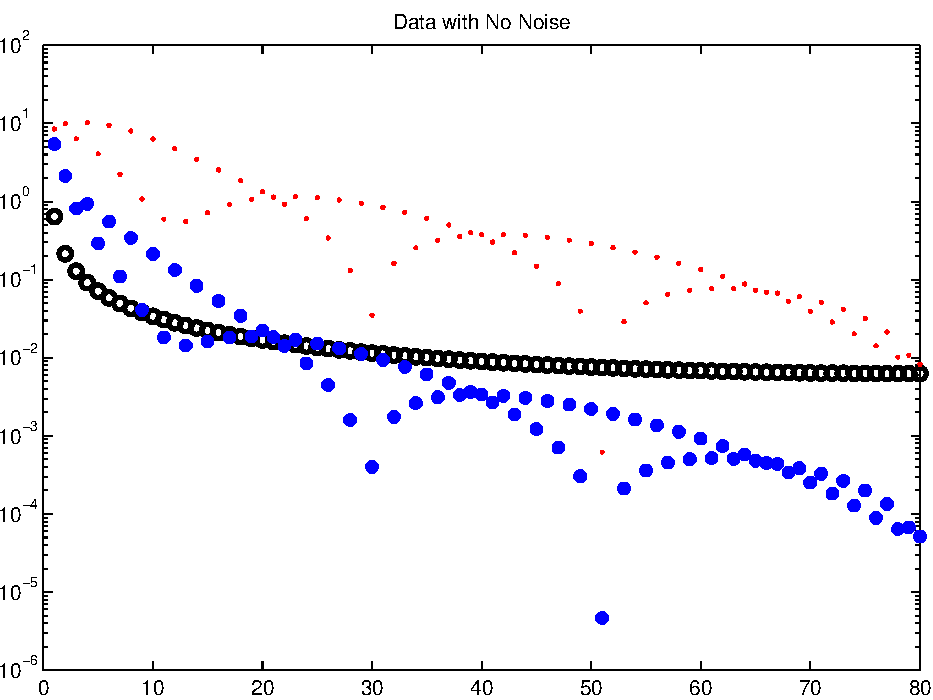
\includegraphics[width=.4\textwidth]{no_noise_picard2.pdf}

\begin{wrapfigure}{l}{.4\textwidth}
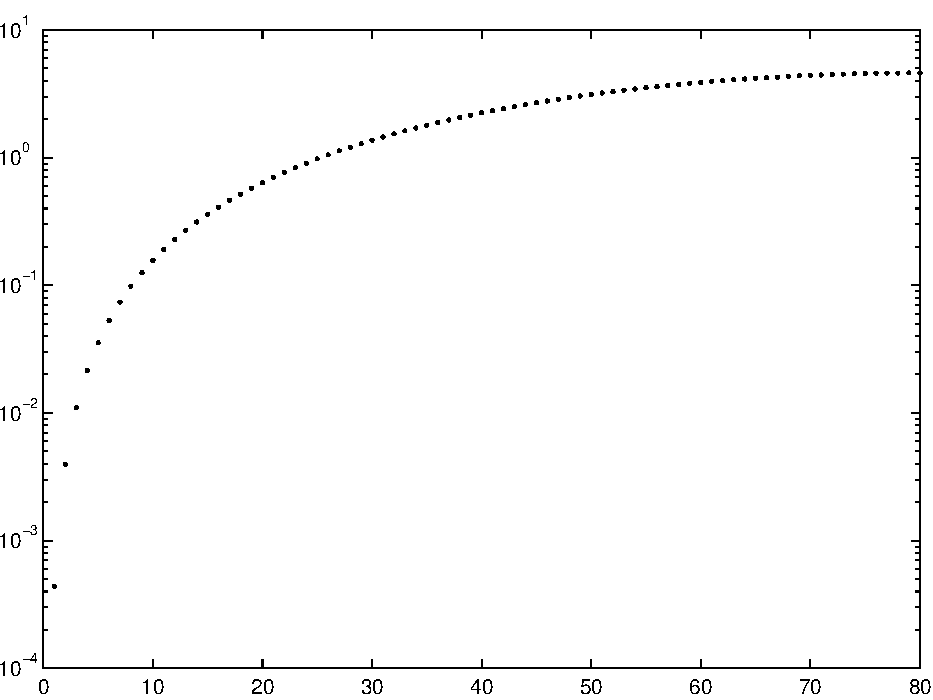
\includegraphics[width=.4\textwidth]{variances2.pdf}
\end{wrapfigure}
 A similar, but less pronounced, exponential increase in the variances $\vect v_i^T \vect x_{\mathrm{LS}}$ is observed.  Note that the ratio in the non-noisy data for this problem does \emph{not} start to increase, indicating that the Picard condition is satisfied for that problem.
\end{longproblem}
\newpage

\begin{longproblem}
\emph{Sampling the least squares solution. }

\subproblem{ Let $\vect v$ be a random $n$-vector with mean $\vect \mu = E[\vect v]$ and covariance
$$
  \vect C = \mathrm{cov}(\vect v) = E\big[ (\vect v - \vect \mu)(\vect v - \vect \mu)^T\big].
$$
Use the linearity of $E$ to show that if $\vect B$ is an $m\times n$ matrix, the mean and covariance of $\vect w = \vect B\vect v$ are $\vect B\vect \mu$ and $\vect{BCB}^T$, respectively.}

\begin{solution}
  Directly from linearity we have that $E[ \vect{Bv} ]= \vect B E[\vect v] = \vect B \vect \mu$.  Using this result, the covariance is given by 
  \begin{align*}
  \mathrm{cov}[\vect{Bv}] &= E\big[ (\vect{Bv} - \vect {B\mu})(\vect{Bv} -\vect {B\mu})^T\big]\\
  &= E\big[ \vect B(\vect{v} - \vect {\mu})(\vect{v} -\vect {\mu})^T\vect B^T\big]\\
  &= \vect BE\big[ (\vect{v} - \vect {\mu})(\vect{v} -\vect {\mu})^T\big]\vect B^T\\
  &= \vect B\vect C\vect B^T\\
  \end{align*}
\end{solution}

\subproblem{ Use part (a) to prove 
$$
  \vect x_{\mathrm{LS}} \sim \mathcal N(\vect x, \sigma^2 (\vect A^T\vect A)^{-1}).
$$
\Hint First show that $\vect x_{\mathrm{LS}} = \vect x + (\vect A^T\vect A)^{-1}\vect A^T\vect \epsilon$, where $\vect \epsilon \sim \mathcal N(\vect 0,\sigma^2 \vect I)$.}

\begin{solution}
  We assume that a linear transformation of a normal random vector is also distributed normally.  

  Since $\vect b = \vect A\vect x + \vect \eps$, we have that $\vect
  x_{\mathrm{LS}} = (\vect A^T \vect A)^{-1} \vect A^T \vect b = (\vect A^T
  \vect A)^{-1} \vect A^T\vect A x + (\vect A^T \vect A)^{-1} \vect \epsilon =
  \vect x + (\vect A^T \vect A)^{-1} \vect A^T \vect \epsilon$.  Recall that $\vect
  \epsilon \sim \mathcal N(\vect 0,\sigma^2 \vect I)$, so by linearity and
  part\nobreak(a), $E[\vect x_{\mathrm{LS}}] = \vect x + (\vect A^T \vect
  A)^{-1}\vect {A0} = \vect x$ and $\mathrm{cov}(\vect x_{\mathrm{LS}}) = \vect 0
  + (\vect A^T \vect A)^{-1}\vect A^T \sigma^2 \vect I \vect A ((\vect A^T \vect A)^{-1})^T = \sigma^2 \vect A^T \vect A$ since $(\vect A^T \vect A)^{-1}$ is symmetric.  I.e. $(\vect A^T \vect A) (\vect A^T \vect A)^{-1} = I$ impies $((\vect A^T \vect A)^{-1})^T (\vect A^T \vect A) = I^T = I = (\vect A^T \vect A) (\vect A^T \vect A)^{-1}$ if and only if $((\vect A^T \vect A)^{-1})^T = (\vect A^T \vect A)$.
  \end{solution}

\subproblem{In the m-file \texttt{TwoVarTest.m}, samples of $\vect
x_{\mathrm{LS}}$ are computed by first sampling $\vect b \sim \mathcal
N(\vect{Ax},\sigma^2\vect I)$ and then computing the corresponding least
squares solution $\vect x_{\mathrm{LS}}$ via the normal equation.  Add a line
of code that also samples $\vect x_{\mathrm{LS}}$ using the approach in part
(b), then plot the two collections of samples together in different colors to
verify that the sample distributions look roughly the same.  Also compare their
sample mean and covariance matrices using MATLAB's \texttt{mean} and
\texttt{cov} functions.}
\begin{solution}
  An example of the the requisite line of code is:
  \begin{lstlisting}
  xx_LS = repmat(x,1,nsamp) + sigma*inv(A'*A)*A'*randn(2,nsamp);
  \end{lstlisting}
Below, we compare the means and covariance matrices of the two distributions,
  \begin{lstlisting}
>> mean(x_LS'),mean(xx_LS') 

ans =

    1.2887    0.7118


ans =

    0.7682    1.2383

>> cov(x_LS'), cov(xx_LS') 
 
ans =

   47.0491  -47.0134
  -47.0134   46.9989


ans =

   50.1726  -50.1840
  -50.1840   50.2155
\end{lstlisting}

  Note that the mean of each solution is relatively far from \texttt{[1 1]'}.
  The initial \texttt{x\_LS} was computed via MATLAB's \texttt{\textbackslash}
  operator, and produces similarly biased results as when using the
  \texttt{inv} function on the standard normal data via the approach in part (b).  Moreover, when using the backslash
  operator to calculate the mean via the approach in part (b), we get this bizarre result
  \begin{lstlisting}
>> xx_LS = repmat(x,1,nsamp) + sigma*(A'*A)\(A'*randn(2,nsamp));  
>> mean(xx_LS') 

ans =

  -24.9983   26.8798
  \end{lstlisting}
  From which, I can only assume that something other than LU decomposition is happening.  In any case, solving for $\vect x$ in $(\vect A^T\vect A) \vect x = \vect b$ is ill-conditioned, and this may be a bi-product of this.

  Below, is the distribution of both methods overlayed on each other.
  \begin{center}
  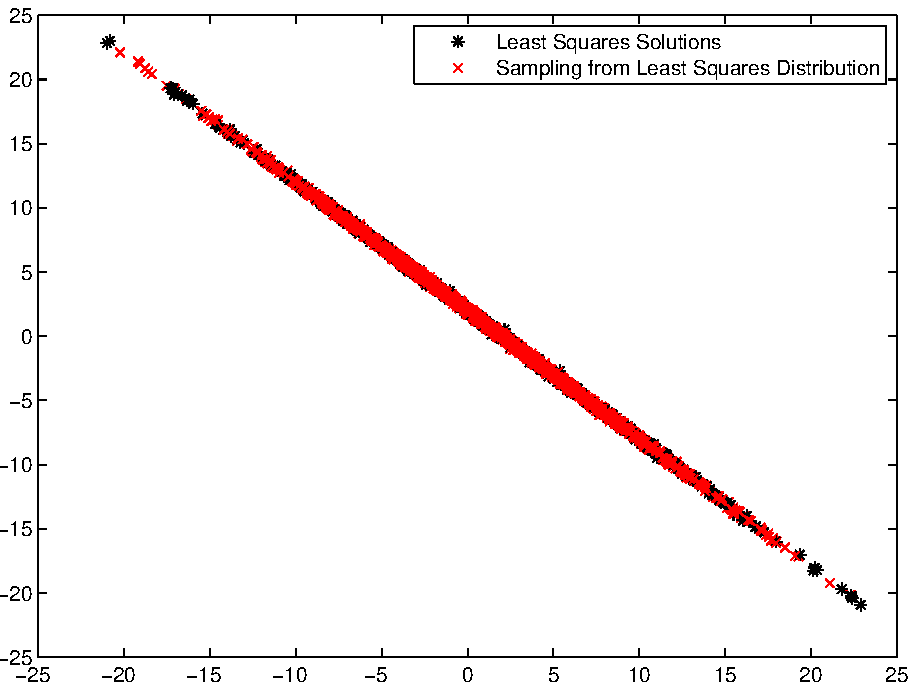
\includegraphics[width=.45\textwidth]{xls_sample.pdf}
  \end{center}
\end{solution}

\subproblem{Create normalized histograms (using the \texttt{hist} function)
from the samples of $\vect v_1^T\vect x_{\mathrm{LS}}$ and $\vect v_2^T\vect
x_{\mathrm{LS}}$ computed in \texttt{TwoVarTest.m} and then graph the resulting
sample probabilty densities together with the analytic true normal densities
given by \eqref{variance}.}
  \begin{center}
  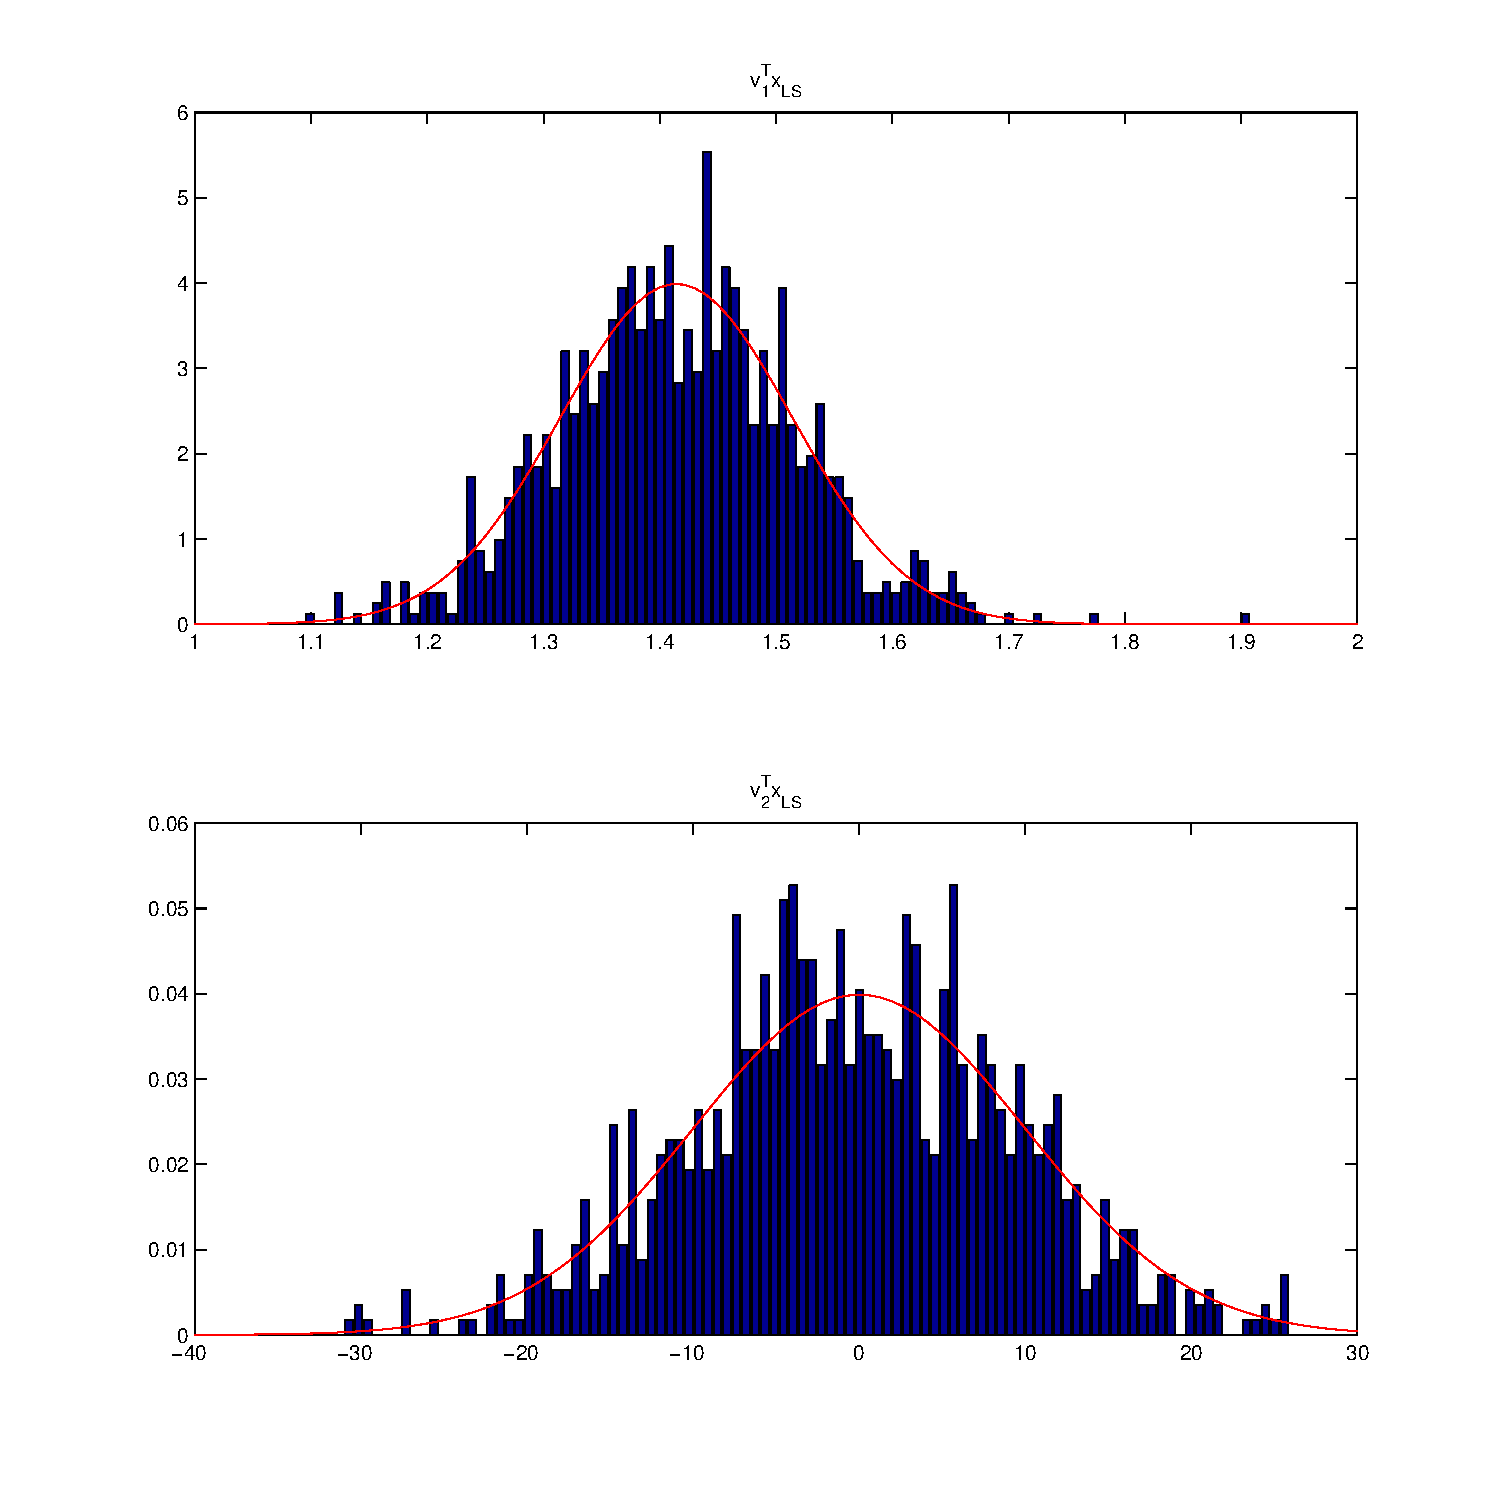
\includegraphics[width=.45\textwidth]{prob_density.pdf}
  \end{center}

The code to produce these is given below
\lstinputlisting[firstline=34,lastline=48]{TwoVarTest.m}

\end{longproblem}
\end{document} 
